% Set the author and title of the compiled pdf
\hypersetup{
  pdftitle = {\Title},
  pdfauthor = {\Author}
}

\section{Terminology}

In order to talk about Strings in any meaningful way, we must first define
terminology that we can use to describe exactly what we mean. What follows is a
list of the terminology used throughout the course:

\begin{itemize}
  \item A {\bf symbol} is basically a letter. They are the basic component of
  all the data we use in the course. Examples include: {\it a, A, (, \$, 7}.
  \item An {\bf alphabet} is a collection of symbols that we can think of as a
  set. Example alphabets may include binary ({\it 0, 1}), Latin letters ({\it
  a,\dots,z,A,\dots,Z}) etc.
  \item A {\bf String} is a collection of symbols from an alphabet grouped
  together, sometimes called a word. Examples include {\it ababa} and
  {\it 100101}.
  \item The {\it empty word} is a String consisting of no symbols. It is
  denoted by the letter $\epsilon$.
  \item {\bf Concentration} an operation that takes two Strings and combines
  them to create one longer String. For example concentrating {\it t} and {\it
  he} would create {\it the}. We can use the power notation to concentrate a
  String with itself any number of times. For example, ${ho}^3$ would give us
  $hohoho$.
  \item A {\bf language} is a collection of Strings that can be thought of as
  a set. Examples of languages could be $\{\emptyset\}$, $\{\epsilon\}$,
  $\{hot,hotter,hottest\}$ or $\{a^n | n \in \mathbb{N}\}$.
\end{itemize}

We also have notation for describing generic instances of such entities:

\begin{center}
  \begin{tabular}{l l}
    {\bf Entity} & {\bf Generic notation}\\
    Symbol & $x, y, z$\\
    Alphabet & $\Sigma$\\
    String & $s, t, u$\\
    Language & $\mathcal{L}$\\
  \end{tabular}
\end{center}

\paragraph{Languages as sets} Since languages are thought of as sets, we can
perform all the usual set operations on them (see my {\tt COMP11120} notes for
more information on these operations). Languages can be concentrated as
described above.

Sometimes, we may want to define any finite number of concatenations of a
language, and this is known as the {\bf Kleene star}. The notation is
$(\mathcal{L})^*$.

An interesting case of this is when a languages is subject to concatenation zero
times ($\mathcal{L}^0$), since this would return the empty word $\epsilon$.

\marginpar{{\it Kleene} is pronounced like {\it genie}.}

\section{Describing languages}

\subsection{Describing languages through patterns}

A pattern describes a generic form that a set of Strings can take. If any String
from the set is compared with the pattern then it will match the pattern. Any
String from outside the set will not match the pattern.

For example, the pattern $(ab)^*$ would match Strings such as $\epsilon$, $ab$,
$abab$, $abab \dots ab$.

\marginpar{$\epsilon$ is matched here since it satisfies the pattern $(ab)^0$.
This comes about because, the Kleene star matches all concatenations of a
String.}

\subsection{Regular expressions}

The terms {\it pattern} and {\it regular expression} are pretty much synonymous.
The operators allowed in a regular expression are:

\begin{center}
  \begin{tabular}{>{\bfseries} l l}
    Empty pattern & The character $\emptyset$ is a pattern.\\
    Empty word & The character $\epsilon$ is a pattern.\\
    Letters & Every letter in $\Sigma$ is a pattern.\\
    \rowcolor{Gray}
    Concatenation & If $x$ and $y$ are patterns, then so is $(xy)$.\\
    \rowcolor{Gray}
    Alternative & If $x$ and $y$ are patterns, then so is $(x|y)$.\\
    \rowcolor{Gray}
    Kleene Star & If $x$ is a pattern, then so is $(x^*)$.
  \end{tabular}
\end{center}

\marginpar{If we were to analyse a pattern in a recursive fashion, then in order
to end our analysis, we would eventually have to find one of a selection of {\it
base cases}.The highlighted rows here represent {\it step cases} (that is to say
that at least another level of recursion is needed to finish our analysis),
while the un-highlighted lines are base cases.}

\subsubsection{Discarding brackets}

Just like in high-school mathematics, brackets can be discarded when
unnecessary. For example, the pattern $((0|1)^*0)$ is equivalent to $(0|1)^*0$,
and $(2|(1|0))$ is the same as $(2|1|0)$.

\subsubsection{Matching a regular expression}

As was implied above, we can define a regular expression by recursively
applying more operators to a `base case' until we have the desired pattern.

The following patterns match the following words:

\begin{center}
  \begin{tabularx}{\textwidth}{>{\bfseries} l X}
    Empty word    & The empty word only matches the pattern $\epsilon$.\\
    Base case     & A pattern $x$ will match a character $x$ where $x$ is
              a member of $\Sigma$\\
    Concatenation   & If $p_1$ is a pattern and $p_2$ is a pattern, then
              $p_1p_2$ will match any word matched by $p_1$
              prepended to and word matched by $p_2$\\
    Alternative   & $(p_1|p_2)$ will match a word from either $p_1$ or 
              $p_2$.\\
    Kleene star   & The pattern $(p^*)$ will match any number of words
              that are matched by $p$ concatenated with each other.
              It also matches the empty word.\\
  \end{tabularx}
\end{center}

\subsection{Languages described by regular expressions}

A language $\mathcal{L}$ described by a regular expression $p$ is one made up of
every word $s$ that is matched by $p$:

\[
  \mathcal{L}(p) - \{s \in \Sigma^* | s~matches~p\}
\]

Obviously, we can describe the same language using different patterns, for
example:

\[
  \mathcal{L}((1|1)(0|0)) = \mathcal{L}(10)
\]

We can find out the exact language defined by a pattern in the following manner:

\[
  \begin{split}
    \mathcal{L}((0|1)(1)^*) &= \mathcal{L}(0|1) \cdot \mathcal{L}(1^*)\\
                &= \mathcal{L}(0) \cup \mathcal{L}(1) \cdot \mathcal{L}(1^*)\\
                &= \mathcal{L}(0) \cup \mathcal{L}(1) \cdot \mathcal{L}(1)^*\\
                &= \{0\} \cup \{1\} \cdot \mathcal{L}(1)^*\\
                &= \{0\} \cup \{1\} \cdot \{1\}^*\\
  \end{split}
\]

\subsubsection{Regular languages}

We say that a language is regular if we can describe the language by defining a
regular expression.

\section{Finite State Automata}

It is often useful to be able to describe languages using pictures. These are
called finite state automata (FSA's). Every FSA must have the following things:

\begin{itemize}
  \item One or more states.
  \item Arrows between states with labels directing the required conditions to
      traverse the arrow.
  \item A start state (indicated by an arrow with it's tail free).
  \item One or more accepting states. If we end up here after traversing the
      automation, then it will match our word.
\end{itemize}

\subsection{Example automata}

Here is an automata that will match the pattern $0(0|1)0$:

\begin{center}
  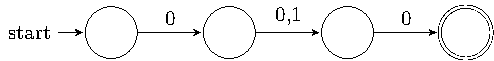
\includegraphics{automata/1.pdf}
\end{center}

If we wanted to, we could include all the {\it dump states} in the automata.
Dump states are states that once entered into, it is impossible to reach an
accepting state. The same automata with a dump state in would look like:

\begin{center}
  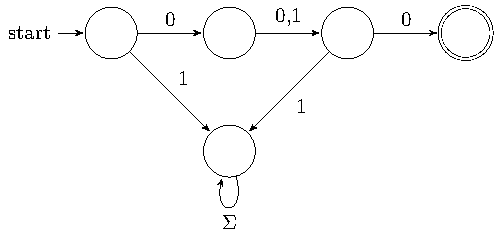
\includegraphics{automata/2.pdf}
\end{center}

\subsection{Formalising the automata}

If we wanted to, we could define the set $Q$ as the set of states in an
automata, and the set $F$ as the set of the accepting states, where $F \subset
Q$. The transitions in the automata could be represented as a function $\delta$,
which takes an input state $s_{in} \in Q$, and a character $c \in \Sigma$, and
returns another state $s_{out} \in Q$.

\[
  \delta:\{(s_{in},c)| s_{in} \in Q, c \in \Sigma\} \rightarrow Q
\]

\marginpar{When an automata is defined like this, it can be seen as a {\it finite
state machine}}

\subsection{Deterministic and non-deterministic automata}

An automata is said to be deterministic if there is only one path through it for
every word in $\mathcal{L}$, however, if there are multiple possible routes
through an automata (i.e. there is no unique path for one or more words), then
we say that the automata is non-deterministic.

Here is an example of a deterministic and a non-deterministic automata that will
accept the language of words defined by the pattern $(0|1)^*(11)$:

\begin{center}
  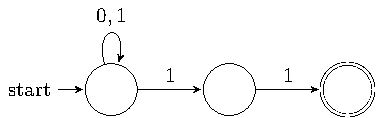
\includegraphics{automata/3.pdf}
\end{center}

\begin{center}
  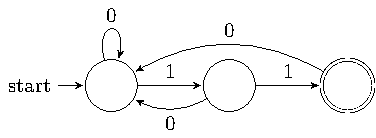
\includegraphics{automata/4.pdf}
\end{center}

\section{Algorithm one}

Algorithm one is a method for converting an NFA to a DFA. In order to do this,
algorithm one walks through an NFA, in a recursive manner, finding all the
possible collections of states that can be reached from each state.
Unfortunately, this behaviour is hard to describe in a general and abstract
manner, so it's probably easiest to just do an example.

\subsection{Algorithm one example}

We'll do Exercise 19 in Andrea's notes, which is to convert the following NFA
into a DFA:

\begin{center}
  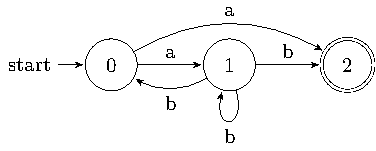
\includegraphics{automata/5.pdf}
\end{center}

In order to apply algorithm one to this automata, we first need to write down
the start state:

\begin{center}
  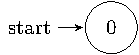
\includegraphics{automata/6.pdf}
\end{center}

From the state $0$, we can go to the state $1$ or the state $2$ with an $a$
transition, therefore algorithm one dictates that we have to create a new state
in our DFA called $12$ that is linked to the state $0$ with an $a$ transition.
Since $2$ is an accepting state in the NFA, then our new state must also be an
accepting state.

\begin{center}
  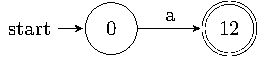
\includegraphics{automata/7.pdf}
\end{center}

Now, we've dealt with the $0$ state, we must concern us with where we can go
from the state $12$. Since this represents both the state $1$ and the state $2$
in the NFA, we must consider the transitions we can do from either of them. From
state $1$ in the NFA, we can go to either state $0$, $1$ or $2$ with a $b$
transition. Concequently, we should make a new state in our DFA for this:

\begin{center}
  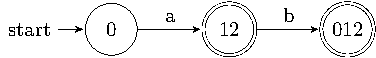
\includegraphics{automata/8.pdf}
\end{center}

From the state $0$, $1$ and $2$, we can go anywhere with a $b$, so we should
make a transition in our DFA for that:

\begin{center}
  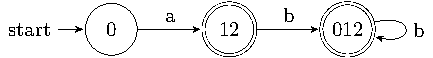
\includegraphics{automata/9.pdf}
\end{center}

From the states $0$, $1$ or $2$ in the NFA, we can go to the states $1$ or $2$
with an $a$ transition:

\begin{center}
  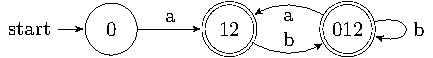
\includegraphics{automata/10.pdf}
\end{center}

\marginpar{If you want a formal definition of algorithm one, take a look at page
33 of Andrea's notes. although it's well explained, I don't think it's worth
including here, since the formal definition won't be very useful in the exam.}

\subsection{Algorithm two}

Algorithm two takes a DFA and converts it into a regular expression. If you want
to convert an NFA into a regular expression, then you must first convert it into
a DFA using algorithm one.

\subsubsection{Numbering states}

Algorithm two relies on us having named all the states in the DFA before we
attempt to apply the algorithm. Although in theory, the algorithm will work with
any state numbering, it is easiest to apply when the states are ordered in {\it
reverse order of complexity}. That is to say that the states with the fewest
connections will have the lowest number.

\marginpar{The numbering of the states isn't vital. If you get one or two the
wrong way round, then it probably won't make the algorithm too complicated.
Also, whether the algorithm is an acceptance state has no bearing on its
number.}

\subsubsection{Applying algorithm two}

First of all, we must determine which states a word from the language
$\mathcal{L}$ accepted by the automation must start and end in. In order to do
this, we must find the start states and all of the possible end states:

\[
	\mathcal{L} = \lang{start}{accepting_0}{} \cup
		\lang{start}{accepting_1}{} \cup \dots \cup \lang{start}{accepting_n}{}
\]

If the automation we were looking at was something like this:


\begin{center}
  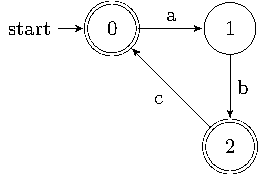
\includegraphics{automata/11.pdf}
\end{center}

Then the language described by the automation would be:

\[
	\mathcal{L} = \lang{0}{0}{} \cup \lang{0}{2}{}
\]

We must now break down this expression into its component parts, $\lang{0}{0}{}$
and $\lang{0}{2}{}$ and evaluate them individualy.

\[
	\begin{split}
		\lang{0}{0}{\leq 2} &= \lang{0}{0}{\leq 1} \cup \left( \lang{0}{2}{\leq 1} \cdot {\lang{2}{2}{\leq 1}}^{*} \cdot \lang{2}{0}{\leq 1} \right)\\
		\lang{0}{0}{\leq 1} &= \epsilon\\
		\lang{0}{2}{\leq 1} &= \lang{0}{2}{\leq 0} \cup \left( \lang{0}{1}{\leq 0} \cdot {\lang{1}{1}{\leq 0}}^{*} \cdot \lang{1}{2}{\leq 0} \right)\\
							&= \emptyset \cup \left( a \cdot \epsilon^*  \cdot b \right)\\
							&= ab\\
		\lang{2}{2}{\leq 1} &= \lang{2}{2}{\leq 0} \cup \left( \lang{2}{1}{\leq 0} \cdot {\lang{1}{1}{\leq 0}}^{*} \cdot \lang{1}{2}{\leq 0} \right)^*\\
							&= \epsilon \cup \left( ca \cdot \epsilon^* \cdot b \right)^*\\
							&= \epsilon | (cab)^*\\
		\lang{2}{0}{\leq 1} &= c\\
		\lang{0}{0}{\leq 2} &= \epsilon | ab(cab)^*c\\\\
		\lang{0}{2}{\leq 2} &= \lang{0}{2}{\leq 1} \cdot {\lang{2}{2}{\leq 1}}^*\\
							&= \{ab\} \cdot \{(cab)^*\}\\
							&= ab(cab)^*\\
	\end{split}
\]

We can now just concatenate the two languages we found and simplify the
resulting regular expression:

\[
	\begin{split}
		\mathcal{L} &= \epsilon | ab(cab)^*c \cup ab(cab)^*\\
					&= \epsilon | ab(cab)^* (c|\epsilon)
	\end{split}
\]

\section{Algorithm three}

The role of algorithm three is to construct a non-deterministic finite automata
from a regular expression.

Algorithm three recursively analyses the regular expression into small chunks of
NFA and then makes use of {\it epsilon transitions} to link these parts
together. 

\marginpar{An epsilon transition is a transition between states in the NFA that
does not require a letter from the word to be traversed. This allows you to join
NFA's together.}

There are a number of general cases in algorithm three, where a regular
expression of a particular form will create an NFA with a certain structure:

\begin{description}
	\item {\bf The empty pattern $\emptyset$}:\\
		A regular expression that accepts no words will produce an NFA like
		this:
		\begin{center}
		  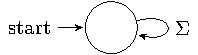
\includegraphics{automata/12.pdf}
		\end{center}
	\item {\bf The $\epsilon$ pattern}:\\
		A regular expression that the empty word will produce an NFA like this:
		\begin{center}
		  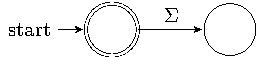
\includegraphics{automata/13.pdf}
		\end{center}
	\item {\bf A pattern accepting a word $x, x \in \Sigma$}:\\
		\begin{center}
		  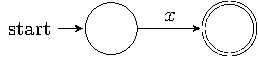
\includegraphics{automata/14.pdf}
		\end{center}
\end{description}

In order to produce a meaningful NFA, we must also handle cases where regular
expressions implement concatenation, alternatives and the kleene star:

\begin{description}
	\item {\bf Concatenation}:\\
		In order to create an NFA that will recognise the same language as a
		pattern that uses concatenation (e.g. $xy$), we must first create two
		NFA's to accept each half of the concetenation, lets call these $X$ and
		$Y$. In order to connect them, we must change all the accepting states
		in $X$ to non-accepting states and make an $\epsilon$ transition from
		them to the start state of $Y$.

		For example:

		\begin{tabular}{lcr}
			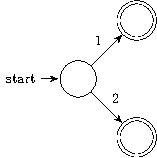
\includegraphics{automata/15.pdf}
			&
			Concatenated with
			&
			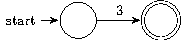
\includegraphics{automata/16.pdf}
		\end{tabular}

		Goes to:

		\begin{center}
		  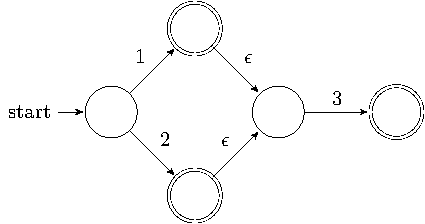
\includegraphics{automata/17.pdf}
		\end{center}
	\item {\bf Alternative}:\\
		To create an NFA that implements an alternative such as $x|y$, then we
		must make a new NFA that has a start state that connects to the other
		NFA's that will accept $x$ and $y$ with $\epsilon$ transitions:

		For example:

		\begin{center}
		  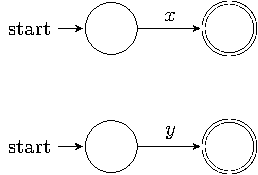
\includegraphics{automata/18.pdf}
		\end{center}

		Combine to make:

		\begin{center}
		  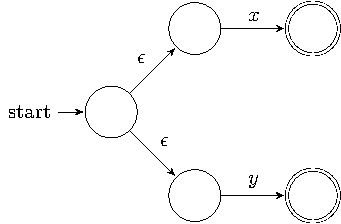
\includegraphics{automata/19.pdf}
		\end{center}

	\item {\bf Kleene star}:\\

		To implement a Kleene star with an NFA, you simply create an epsilon
		transition from each accepting state in the NFA to the start state, and
		make sure that the start state is an accepting state.

		For example:

		\begin{center}
		  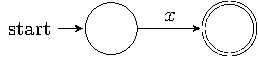
\includegraphics{automata/20.pdf}
		\end{center}

		Goes to:

		\begin{center}
		  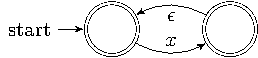
\includegraphics{automata/21.pdf}
		\end{center}


\end{description}